\section{Grundlagen} % (fold)
\label{sec:grundlagen}
	
	
	\subsection{$\gamma$-Strahlung} % (fold)
	\label{sub:entstehung_un_deingeschaften_von_gamma_strahlung}
		
		Es gibt zwei Kriterien, nach denen sich elektromagnetische Strahlung in den Bereich der $\gamma$-Strahlung einteilen lässt.
		Geht man nach Energie und Wellenlänge, so befindet sich $\gamma$-Strahlung im Spektrum im Bereich von circa $10^{18}$ bis $10^{23} \unit{Hz} $ also im Wellenlängenbereich von $300$ bis $0.003 \unit{pm} $ beziehungsweise bei Quantenenergien von rund $10 \unit{keV}$ bis $1 \unit{GeV}$.
		Damit überschneidet sich das $\gamma$-Spektrum am unteren Rand mit dem der harten Röntgenstrahlung.
		Als eigentliches Kriterium dient deshalb auch eher die Entstehung der Strahlung.
		Während Röntgenstrahlung noch durch elektronische Übergänge in der Atomhülle beziehungsweise durch Bremsstrahlung entsteht, wird $\gamma$-Strahlung stets bei Kernprozessen frei.
		Am Anfang steht dabei immer eine Kernumwandlung, also Spaltung, Teilcheneinfang, $\alpha$-, oder $\beta$-Zerfall.
		Die Reaktionsprodukte sind meistens immer noch angeregte Kerne, die nach einiger Zeit in den Grundzustand zurückfallen und ihre restliche Energie dabei in Form eines $\gamma$-Quants abgegeben.
		Ein solches Zerfallsschema ist in Abbildung \ref{fig:dec-scheme} zu sehen.

		\begin{figure}[htb]
			\centering
			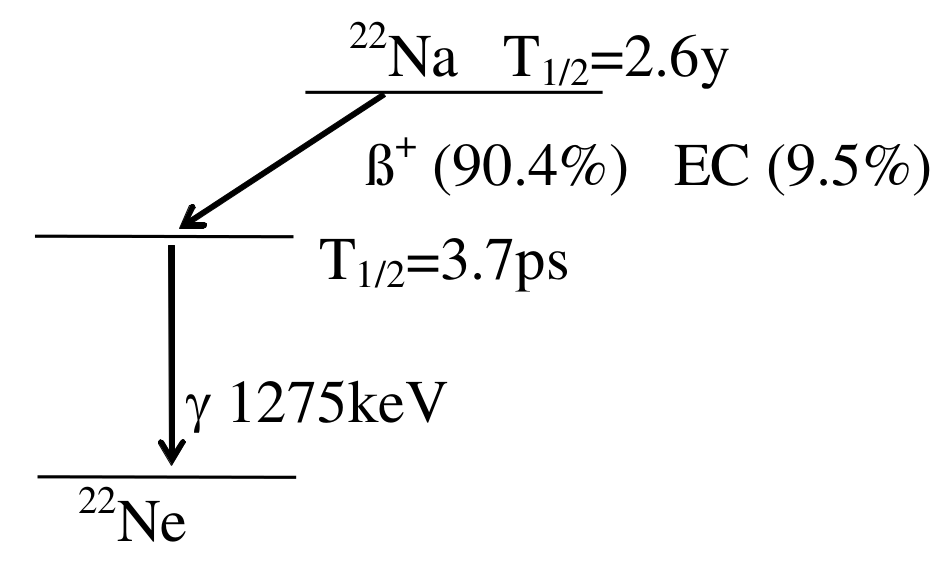
\includegraphics[scale=0.28]{pic/na-22-decay-scheme.png}
			\caption{ $\beta^+ $-Zerfallsschema des $ \prescript{22}{}{\m{Na}} $ mit zugehörigen Energie und Halbwertszeiten \\
			Quelle: Versuchsvorbereitung}
			\label{fig:dec-scheme}
		\end{figure}

		Eine andere Möglichkeit ist die Zerstrahlung von Antimaterie (welche meist auch erst durch Kernprozesse entsteht).
		Dabei treffen zum Beispiel ein Elektron und ein Positron aufeinander, annihilieren und setzen zumeist zwei Quanten frei, deren Energie jeweils der Ruheenergie einer der beiden Reaktionspartner entspricht, also in diesem Fall $511 \unit{keV}$.

	% subsection entstehung_un_deingeschaften_von_gamma_strahlung (end)
	
	

	\subsection{Wechselwirkung mit Materie} % (fold)
	\label{sub:wechselwirkung_von_gammastrahlung_mit_materie}	
	
		Für den Versuch sind vor allem drei Arten der Wechselwirkung von $\gamma$-Strahlung mit dem Detektormaterial relevant.


		\subsubsection{Der Photoeffekt}
		\label{sssec:photoeffekt}
		
			Ein Photon, dass die notwendige Mindestenergie besitzt, kann ein Elektron aus der Atomhülle anregen und wird dabei vollständig absorbiert.
			Vernachlässigen wir die Ionisierungsenergie des Elektrons (meist im eV bis keV-Bereich), welche durch das $\gamma$-Quant bei weitem überschritten wird, so hat das Elektron im Anschluss in etwa kinetische Energie des Photons.
			Da Elektron und Photon unterschiedliche Energie und Impulsbeziehungen haben, aber beide Erhaltungssätze gelten, muss das Atom den überschüssigen Impuls aufnehmen.
			Photoeffekt tritt daher bevorzugt bei stark gebundenen Elektronen und kleineren Photonenenergien auf.
			Für den Wirkungsquerschnitt $\sigma_{\m{ph}}$ gilt
			\[ \sigma_{\m{ph}} \sim Z^5 / E_\gamma \]  
		
		% subsubsection photoeffekt


		\subsubsection{Der Compton-Effekt}
		\label{sssec:comptoneffekt}
		
			Trifft ein $\gamma$-Quant auf ein freies oder schwach gebundenes Elektron, so kommt es meist zur inelastischen Streuung, auch Compton-Streuung genannt.
			Dabei überträgt das Photon einen Teil seines Impulses und damit auch seiner Energie auf das Elektron.
			Die Impuls- und damit auch die Wellenlängenänderung $\Delta \lambda$ des Quants ist abhängig vom Streuwinkel $\varphi$ und wird durch folgende Formel ausgedrückt.
			\[ \Delta \lambda = \lambda_\m{C} (1 - \cos \varphi),\qquad \lambda_\m{C} \define \frac{h}{m_e c} \]
			Je nach Streuwinkel sind somit unterschiedliche Energieüberträge möglich, jedoch gilt gilt für die maximal übertragene Energie $E_\neg$
			\[ \varphi = 180^\circ \quad \implies \quad E_\neg = \frac{E_\gamma}{1 + \frac{m_e c^2}{2 E_\gamma} } \]
			Für hohe Photonenenergien ($E_\gamma > m_e c^2$) gilt für den Wirkungsquerschnitt $\sigma_\m{C}$ näherungsweise:
			\[ \sigma_\m{C} \sim Z / E_\gamma \]
		% subsubsection comptoneffekt


		\subsubsection{Paarbildung}
		\label{sssec:paarbildung}
		
			Bei sehr hohen Photonenenergien $E_\gamma > 2 m_e c^2$ ergibt sich eine dritte Möglichkeit der Wechselwirkung -- die Paarbildung.
			Hierbei erzeugt ein $\gamma$-Quant im Coulombfeld eines Atoms ein Elektron-Positron-Paar.
			Um die Impulsbilanz auszugleichen muss das Atom den übrigen Impuls aufnehmen.
			Das Quant verschwindet bei diesem Vorgang.
			Positronen haben in Gegenwart von Materie eine sehr kurze Lebenszeit.
			In Festkörpern werden sie meist nach wenigen Picosekunden bis Nanosekunden abgebremst und annihilieren mit einem Elektron zu zwei $\gamma$-Quanten mit jeweils der Energie von $m_e c^2 = 511 \unit{keV}$.
			Die Wahrscheinlichkeit der Paarbildung steigt mit der Energie $E_\gamma$, sowie mit der Kernladungszahl $Z$ des beteiligten Atoms, für den Wirkungsquerschnitt $\sigma_\m{P}$ kann man abschätzen:
			\[ \sigma_\m{P} \sim Z^2 \ln E_\gamma \]
		
		% subsubsection paarbildung

		Wie gezeigt haben alle drei Vorgänge unterschiedliche Wirkungsqueschnitte.
		Die Anteile der Effekte an der Absorbtion von $\gamma$-Strahlung in Blei sind in Abbildung \ref{fig:pb-absorb} gegenübergestellt.
		Wie man erkennt sind die jeweiligen Effekte stark von der Energie $E_\gamma$ abhängig.

		\urldef{\refPbAbsorb}\url{https://upload.wikimedia.org/wikipedia/commons/f/f1/Gamma_Abs_Pb.png}
		\begin{figure}[htb]
			\centering
			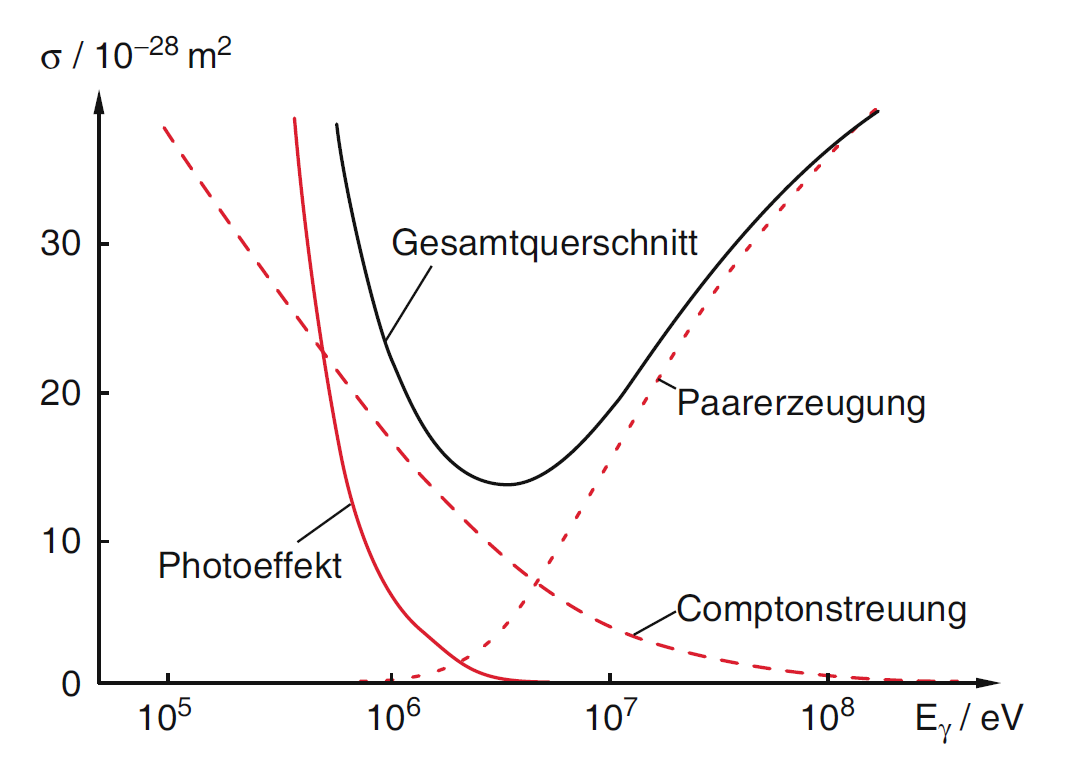
\includegraphics[scale = 0.4]{pic/sigma-funktion.PNG}
			\caption{Wirkungsquerschnitt $\sigma_{ph}$ für Photoeffekt, $\sigma_C$ für Compton-Effekt und $\sigma_P$ für Paarbildung für Blei ($Z = 82$) als Funktion der $\gamma$-Energie}
			\label{fig:pb-absorb}
		\end{figure}

		\begin{figure}[htb]
			\centering
			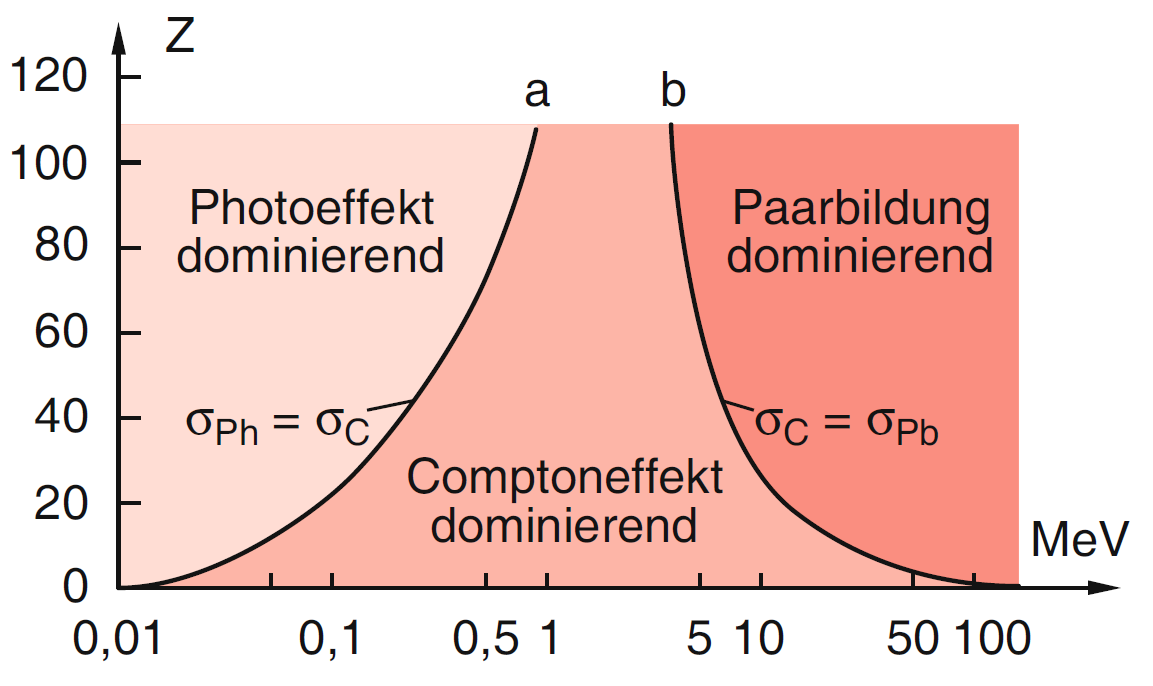
\includegraphics[scale = 0.35]{pic/sigma-bereiche.PNG}
			\caption{Die dominanten Bereiche für Photoeffekt, Compton-Effekt und Paarbildung als Funktion der Ordnungszahl $Z$ des Absorbers und der Energie $E_\gamma$ der $\gamma$-Quanten}
			\label{fig:sigber}
		\end{figure}

		% Die jeweils dominierenden Bereiche sind auch gut in Graph 2222222222222222222 zu sehen.

		% 2GRAPHEN

	% subsection wechselwirkung_von_gammastrahlung_mit_materie (end)


	\subsection{$\gamma$-Spektroskopie} % (fold)
	\label{sub:gamma_spektroskopie}
		
		Bei der $\gamma$-Spektroskopie macht man sich die ionisierende Wirkung der Strahlung zu Nutze.
		Bei allen im Versuch verwendeten Detektoren wird die $\gamma$-Energie des einfallenden Photons zunächst durch den Photo- oder Comptoneffekt auf ein Elektron übertragen.
		Während $\gamma$-Quanten Materie auch ohne Wechselwirkung durchdringen können, verbleiben die Elektronen fast immer im Festkörper.
		Diese sogenannten Primärelektronen erzeugen dann je nach Typ des Detektor ein Signal dessen Stärke proportional zur aufgenommenen Energie ist.
		Dazu gibt es verschiedene Strategien.

		\subsubsection{Germaniumdetektor}
		\label{sssec:ge-detektor}
		
			Der HP-Ge-Halbleiterdetektor (HP für \textbf{H}igh \textbf{P}urity) besteht aus einer in Sperrrichtung betriebenen und gekühlten Ge-Diode. 
			Somit herrscht im Normalfall kein Stromfluss.
			Das angeregte Primärelektron gibt nun seine Energie durch die Erzeugung von Elektron-Loch-Paaren ab.
			Diese wiederum ermöglichen einen Stromfluss.
			Das gemessene Signal ist umso stärker, je großer die Elektronenenergie und damit die ursprüngliche $\gamma$-Energie war.
			Es wird verstärkt und auf einem Vielkanalanalysator gemäß seiner Stärke eingeteilt.
			Die Kühlung verringert das thermische Rauschen des Detektors.

		% subsubsection ge-detektor


		\subsubsection{Szintillationsdetektor}
		\label{sssec:szintillationsdetektor}
		
			Szintillationsdetektoren wie der Plastik-Detektor oder der NaI(Tl)-Detektor nutzen strahlende Übergänge ihrer Bandstruktur zur Signalerzeugung.
			Das Primärelektron regt je nach Energie eine bestimmte Anzahl von Atomen in einem genau definiertem optischen Übergang an, welche nach kurzer Zeit wieder relaxieren und die Energie in Form eines Photons der Bandlückenenergie abgeben.
			Dieses hat im Festkörper keine hohe Reichweite, da es ja genau der Bandlückenenergie entspricht und somit wieder von anderen Atomen absorbiert werden kann.
			Aus diesem Grund werden in geringer Konzentration Fremdatome eingebracht wie z.B. Tellur im Fall von NaI.
			Das Tellur liefert im Festkörper eine Energieniveau, welches tief in der Bandlücke also etwa auf der Hälfte liegt.
			Dadurch kann es zwar durch die NaI-Photonen angeregt werden, die Tl-Photonen können ihrerseits aber keine NaI-Übergänge anregen und passieren den Festkörper somit weitgehend ungehindert.
			Sie treffen nun auf einen Photomultiplier, dessen Signal dann wieder im Vielkanalanalysator zugeordnet und ausgewertet wird.
		
		% subsubsection szintillationsdetektor
	% subsection gamma_spektroskopie (end)
% section grundlagen (end)